\section{Introduction}
\label{sec:intro}

Public spaces in large cities are increasingly becoming complex and unwelcoming environments because of the overcrowding and complex information in signboards. It is in the interest of cities to make their public spaces easier to use, friendlier to visitors and safer to increasing elderly population and to the people with disabilities.

In the last decade, we observe tremendous progress in the development of robots in dynamic environments %with presence of
including people. The new challenge for the near future is that robots will be deployed in public areas (malls, touristic sites, parks, etc.) to offer services to make the use of the environment welcoming and easy to use by visitors, elderly or disabled people. 

Such application domains require robots with new capabilities leading to new scientific challenges: robots should assess the situation, estimate the needs of people, socially interact in a dynamic way and in a short time, with many people, the navigation should be safe and respects the social norms. These capabilities require new skills including robust and safe navigation, robust image and video processing, short-term human-robot interaction models, human need estimation techniques and distributed and scalable multi-agent planning.

\begin{figure}[t!]
\centering
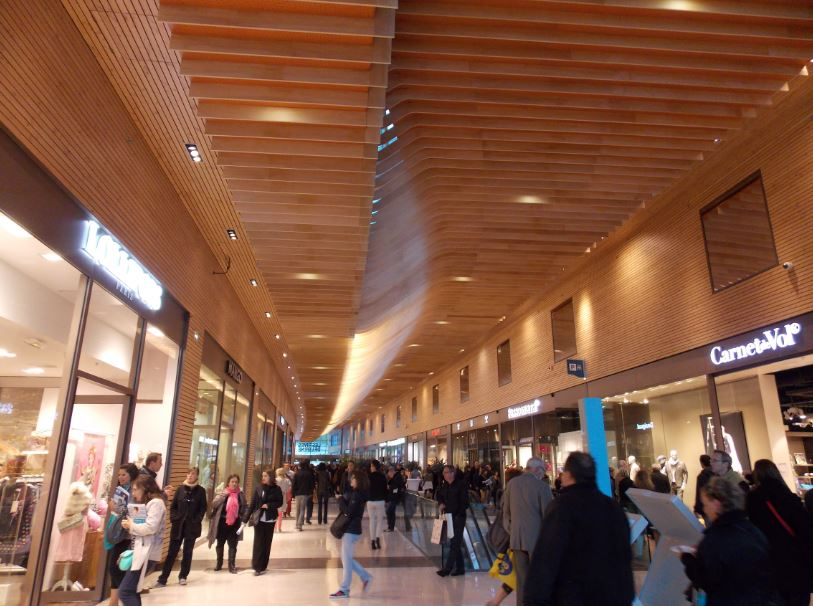
\includegraphics[width=0.65\textwidth]{fig/rivedelorne}
\hspace{0.8cm}
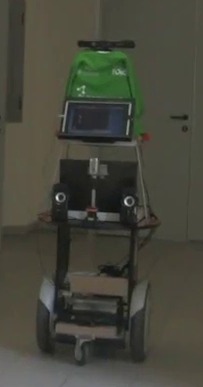
\includegraphics[width=0.255\textwidth]{fig/diago1}
\caption{\coaches environment and robot.}
\label{fig:env}
\end{figure}

In the \coaches project, we aim at further developing this technology, but specifically study, develop and test integration of Artificial Intelligence and Robotics technology in order to develop robots that can suitable interact with users in a complex large public environment, like a shopping mall.
Figure \ref{fig:env} shows the \emph{Rive de l'orne} shooping mall in Caen (France) where the experimental activities of the project will be carried out, as well as a prototype of the robot that will be used.

Previous work on social robotics and human-robot interaction mostly focused on one-to-one human-robot interaction, including elderly assistance (e.g., GiraffPlus project \cite{CoCe14}) and interaction with children (e.g., MOnarCH project \cite{FeSe14}). Robots acting as museum tour-guides have also been successfully experimented. One of the first robot interacting with many non-expert users was RHINO deployed at the ``Deutsches Museum'' in Bonn,
Germany \cite{BuCr98}. In this work, the main focus was in the mapping, localization and navigation abilities in crowded environment, while human-robot interaction was limited to buttons on the robot, a remote Web interface and pre-recorded sentences issued by the robot.

As shown in the figure, in contrast with previous work on social robotics and human-robot interaction, the \coaches environment is very challenging, because populated by many people.
Moreover, we aim at a more sophisticated interaction using multiple modalities (speech, gesture, touch user interfaces) and dialog generated on-line according to the current situation
and the robot's goals.
Consequently, the required level of ``intelligence'' of the \coaches robots in order to adequately perform complex and effective tasks in this environment in presence of people is much higher than in previous projects.

The \coaches project (October 2014 - September 2017) will provide important insights for actual deployment of intelligent social robots in large populated public areas. 
In this paper, we describe the main overall architecture of the system (Section 2), mostly focusing on the components that implement the integration between Artificial Intelligence and Robotics techniques (Section 3): 1) knowledge representation for the semantic map of the environment,
2) planning under uncertainty using MDP, 3) hierarchical task structure for plan execution and monitoring. 
Moreover, in Section 4 we present some preliminary results of such an integration, showing the feasibility of the proposed architecture.



